
\documentclass[twoside]{article}

%\usepackage{scvrt1516}

\usepackage[T2A]{fontenc} 
\usepackage[utf8]{inputenc}
\usepackage[english,russian]{babel}
\usepackage{graphics}
\usepackage{amssymb}
\usepackage{multicol}
\usepackage{mathtext}
\usepackage{amsmath}
\usepackage{graphicx}
\usepackage{multirow}
\usepackage{cite}
\usepackage[hidelinks]{hyperref}
\usepackage{epstopdf}

%\graphicspath{imageEps}

\voffset=-10mm

%The format of the papers: plain text. Volume: 15.000 characters and 5 tables and figures in total.

\begin{document}
\title{Visual inspection of skiing course and terrain using virtual and augmented reality}

\author{
	{Aleshin V., Chuvilin K., Khlamov M., Klimenko S., Klimenko A., Rudskaya E.}
}
\date{}
\maketitle

\section{Введение}\label{intro}

%eng
The study of visual perception and physical actions integration constitute fundamental scientific interest ~\cite{Bulthoff-bib1}.
This work relies on methods well described in (Aleshin et al., 2012).
The significant miniaturization and mobility of modern 3D virtual environment (VE) devices make the appropriate equipment easy to use directly on a ski course. 
The virtual visual inspection of a course and a difficult relief with the use of mobile VE devices is actual for professional sports, freeride, extreme skiing.

%rus
Проблема визуального восприятия является фундаментальной научной задачей ~\cite{Bulthoff-bib1}.
Данная работа опирается на результаты, описанные в ~\cite{Aleshin-2012-bib2} и продолжает серию работ по изучению 3д восприятия в виртуальной
среде.
В качестве примеров 3д сцен выбраны горнолыжные трассы, внетрассовые спуски, фрирайд, так как получение возможности провести виртуальный осмотр трассы 
и сложного рельефа с помощью мобильных устройств является весьма актуальным для профессиональных спортсменов и фрирайдеров.
Значительное уменьшение современных устройств, позволяющих отображать виртуальное окружение позволяет использовать их напрямую на горнолыжных трассах.

\subsection{Motivation}
Воспросы зрения и визуального восприятия исследуются учеными уже довольно давно.
The problems of human 3D perception have been investigated for a long time starting with the pioneer works of V.\;Rauschenbusch~\cite{Rauschenbusch-bib3}.
Стоит также отметить работы Д. Хьюбела и Т. Визеля ~\cite{Hubel-1988-bib4, Hubel-Wiesel-bib5}.
В любительском и профессиональном спорте также уделяется внимание проблемам из этой области.
Изучению визуального восприятия и использованию систем виртуального окружения также посвящен ряд работ ~\cite{Zaichkowsky-2012-bib6, Bideau-2010-bib7}

Горные лыжи, как и любой другой экстремальный вид спорта, связаны с риском.
Международная федерация лыжного спорта уделяет большое внимание вопросам безопасноти на склонах.
10 правил поведения на склоне ~\cite{fis-10-rules-bib8} дают рекомендации лыжникам и сноубордистам, 
следование которым повышает безопасность на склонах.
Но в них неявно подразумевается, что лыжник знает трассу, ее особенности, может адекватно оценивать свои возможности, 
влияние на катание погодных условий и другие факторы.
Однако это не всегда верно, особенно для начинающих лыжников.
Профессионалы также внимательно следят за развитием технологии виртуального окружения.
Например, Линдси Вонн, олимпийская чемпионка в скоростном спуске, отмечает, что эта технология,
которая поможет визуализировать трассу перед спускам, будет очень полезна новичкам, но и также 
отнимет у нее преимущество перед конкурентами: 
"В чём я действительно ощущаю себя сильнее других – это визуализация трассы в мозгу. 
Я способна «прокручивать» все трассы даже летом, хотя и не катаюсь по ним на лыжах."
%http://www.ski.ru/az/blogs/post/proiti-po-grani-intervyu-lindsi-vonn-o-sovremennykh-tekhnologiyakh/

\subsection{Research questions}
Таким образом, задача построения виртуального окружения, предоставляющего возможность лыжникам и сноубордистам
производить предварительный осмотр горнолыжного склона, является актуальной.
Большая часть данного исследования будет посвящена вопросам разработки и использования такого приложения.
Список требований к приложению:

\begin{enumerate}
	\item Осуществление предварительного осмотра реальной трассы.
	\item Просмотр трассы прямо на склоне.
	\item Работа с моделями реальных склонов и трасс.
\end{enumerate}


\section{Method}\label{method}
Системы виртуального окружения включают в себя аппаратную и программную части.
На данный момент существует множество решений и их комбинации для обоих частей.
Задачи данного исследования накладывают некоторые ограничения на возможное решение.
Далее будут описаны аппаратные и программные решения, использованные в проекте.

\subsection{Hardware equipment}
Требования к аппаратной части проекта:

\begin{enumerate}
	\item Компактность. Необходимо иметь возможность использовать систему на спуске.
	\item Дешевизна. Система должна быть достпуна как для профессиональных спортсменов, так и для любителей.
	\item Качество рендеринга. Система должна обеспечивать качество рендеринга, приемлимое для приложений виртуальной реальности.
		Эти требования сейчас выше по сравнению с аналогичными non-VR системами. Например, необходимо обеспечить 
		минимальную частоту смены кадров в секунду (fps) на уровне 90 fps, чтобы изобрадение не начинало дрожать или воспроизводиться с задержками.
\end{enumerate}

На данный момент существует множество вариантов систем виртуальной реалисть, среди которых требованиям проекта полностью удовлетворяют
шлемы виртуальной реальности (HMD).
Первые варианты шлемов виртуальной реальности появились в 2012 году, когда id Software представили прототип Oculus Rift.
Этому шлему было необходимо подключение к ПК, на котором и производились все вычисления.
Однако с развитием мобильных устройств стало возможным создание шлемов виртуальной реальности на их основе.
В такой системе мобильное устройство берет на себя работу по предобработке, рендерингу виртуальной сцены и получению и отправки данных
встроенной системы трекинга.
Сейчас на рынке существует множество вариантов таких шлемов.
Основное отличие между ними лежит в списке возможных совместимых смартфонов и качестве материалов.
Принцип работы этих устройств очень похож.
Два изображения, формирующие стереопару, отображаются на экране смартфона.
Далее каждое из них проходит через линзу, используемую для увеличения угла обзора.
В некоторых устройствах есть возможность изменять расстояние между экраном и линзами.

\begin{figure}[h]
	\centerline{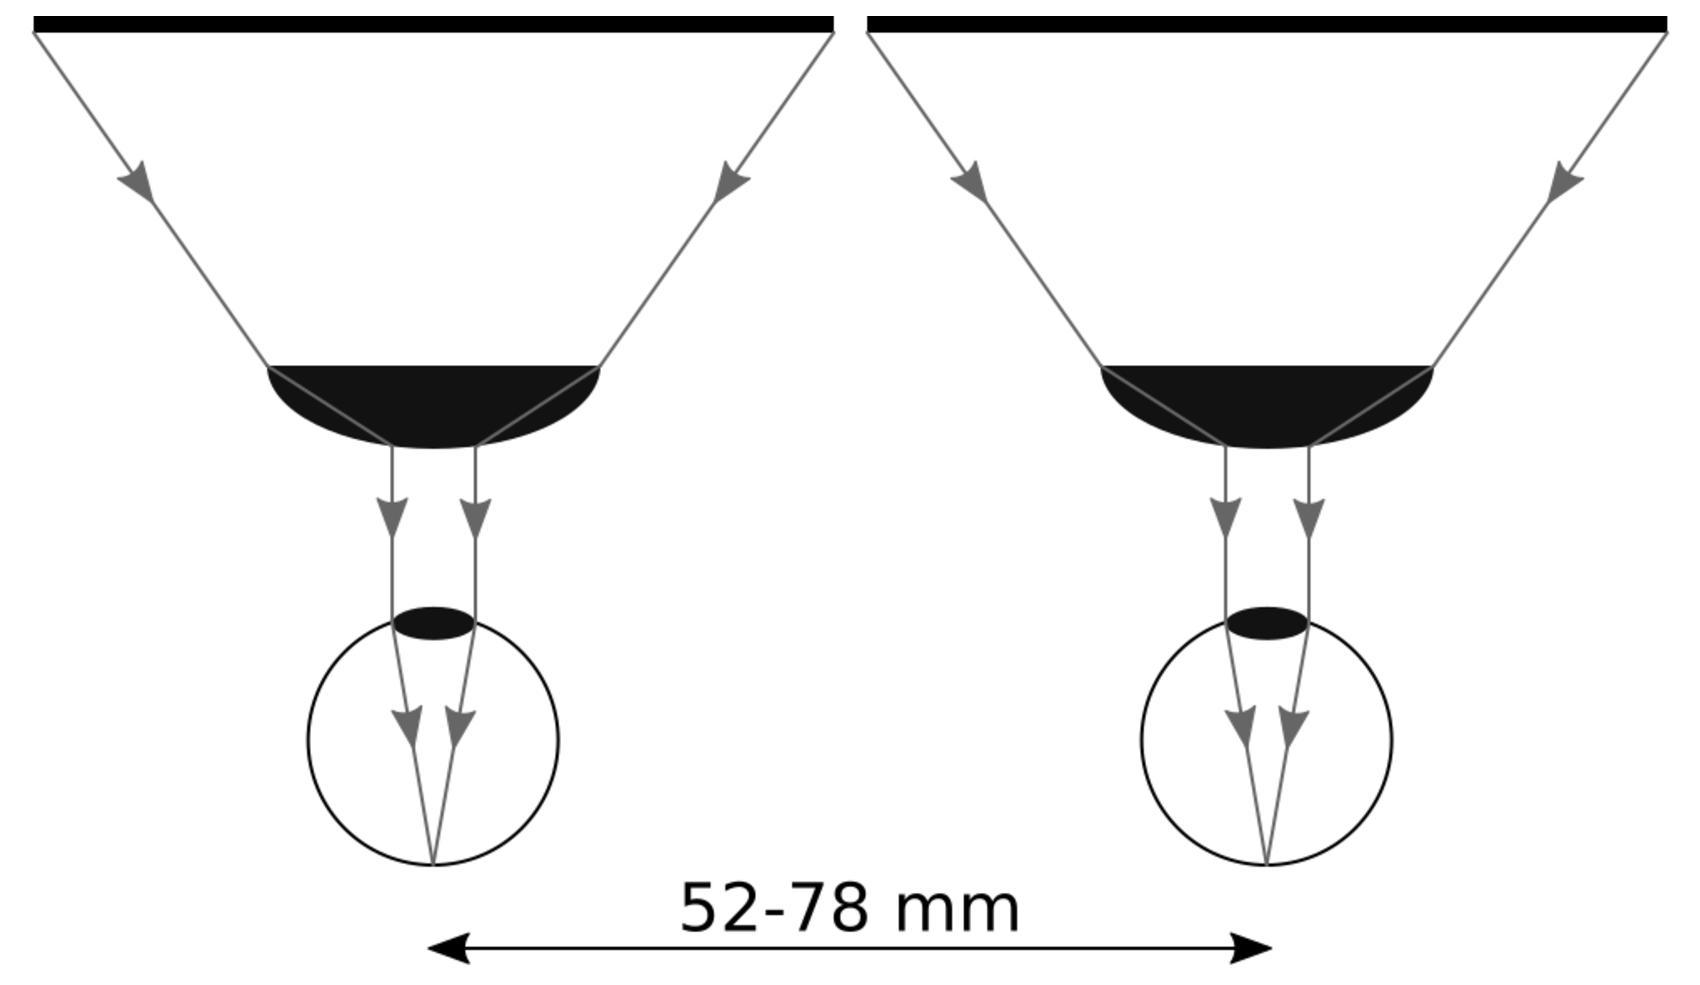
\includegraphics[width=8.5cm]{helmet-scheme.eps}}
	\caption{Principal VR-helmets design}
	\label{figure:helmet-scheme}
\end{figure}

В нашем проекте выбор пал на Samsung Gear VR и Fibrum и смартфон Samsung Galaxy S6.
Данный смартфон обеспечивает достаточную производительности, а сами шлемы достаточно малы, что позволяет использовать их даже на склоне.

\subsection{Software tools}
Для реализации программной части был использован Unity~\cite{unity3d-bib9}.
Этот движок используется нами также и в смежных проектах.
В работе ~\cite{Khlamov-fruct18-bib10} приводится сравнительна характеристика средств, использующихся для разработки
приложений виртуальной реальности и обосновывается выбор Unity.

Основной частью приложения является модель горлолыжного склона.
Unity поддерживает множество форматов 3d-моделей, поэтому необходимые модели трасс можно получить разными способами:
использовать созданные и выложенные в открытый доступ, либо созданные с помощью метода фотограмметрии.
Для получения моделей трасс последним способом использовались фотографии, сделанные с помощью квадрокоптера.
Для построения модели необходимо сделать примерно 50(?) фотографий разрешением X на Y(?).
Затем полученные фотографии обрабатываются в специальном ПОб в нашем случае - Agisoft Photoscan.

\begin{figure}[h]
	\centerline{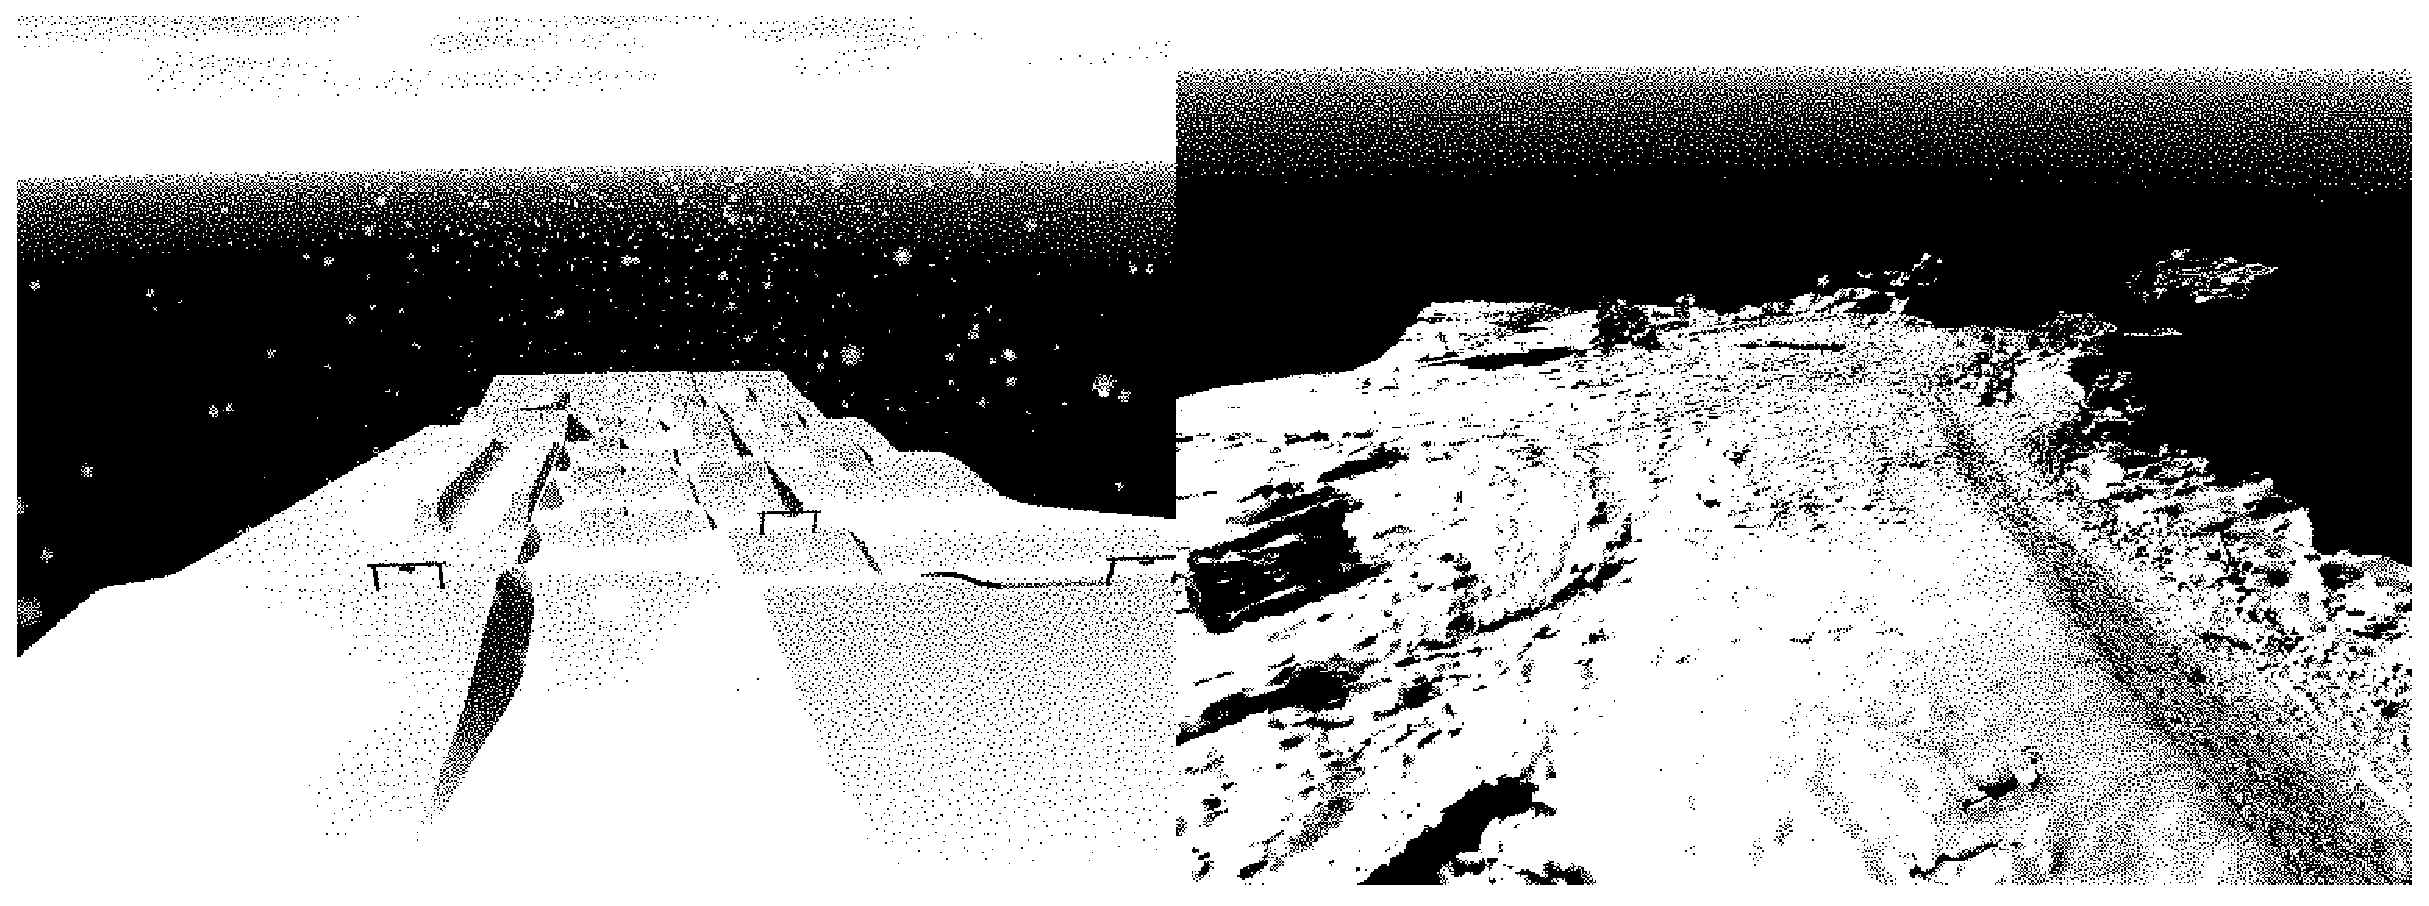
\includegraphics[width=8.5cm]{2slopes.eps}}
	\caption{Модель абстрактной трассы (слева) и реального склона(справа)}
	\label{figure:2slopes}
\end{figure}

(? чем лучше дополнить секцию про фотограмметрию?)

\section{Results}\label{results}

(? Какие результаты писать? МОжет быть успеем провести какие-либо опыты и замерить время/что-то, что можно подсчитать?)


\section{Discussion}\label{discussion}


\section{Conclusion}\label{conclusion}

\vspace*{-2mm}
\begin{thebibliography}{99}
\itemsep=-2pt

\bibitem{Bulthoff-bib1}
	Heinrich Bülthoff, Going beyond vision: multisensory integration for perception and action, // ICVS 2008,Santorini, May 12 2008

\bibitem{Aleshin-2012-bib2}
	Vladimir Aleshin, Stanislav Klimenko, Alexander Bobkov, Dimitrij Novgorodtsev (2012), A Visual 3d Perception Of The Ski Course And Skiing Results, // Proc. of the 5th ICSS 2010, St. Christoph, Austria, 59-68.

\bibitem{Rauschenbusch-bib3}
	B.\,V.\;Rauschenbach,
	\emph{Perspective systems in art. The general theory of perspective
	[``Sistemyi perspektivyi v izobrazitelnom iskusstve. Obschaya teoriya perspektivyi'']},
	Moscow, Nauka, 1986. (in Russian)

\bibitem{Hubel-1988-bib4}
	David H. Hubel, (1988 ), Eye, Brain and Vision, Scientific American Library. F Division of HPHLP, New York, 239p.

\bibitem{Hubel-Wiesel-bib5}
	David H. Hubel, Torsten N. Wiesel, (2005), Brain and Visual  Perception. The Story of 25 - Year Collaboration, Oxford, University Press, 826p.

\bibitem{Zaichkowsky-2012-bib6}
	L.\;Zaichkowsky, J.\;Faubert, P.\;Beauchamp,
	``Visual Perception Training: Cutting Edge Psychophysics and 3D Technology Applied to Sport Science'',
	\emph{Association for Applied Sport Psychology Proceedings},
	2012, Atlanta, Georgia.

\bibitem{Bideau-2010-bib7}
	Bideau B, Kulpa R, Vignais, N, Brault, S, Multon, F \& Craig CM, (2010), Virtual reality, a serious game for understanding performance and training players in sport. IEEE Computer 		Graphic Applications, 30, pp.14-21.

\bibitem{fis-10-rules-bib8}
	FIS rules,
	Web:~\url{http://www.fis-ski.com/mm/Document/documentlibrary/Administrative/04/22/77/10fisrulesforconductsafetyandtheenvironment_newFISCI_Neutral.pdf}

\bibitem{unity3d-bib9}
	Unity 3D official website,
	Web:~\url{http://unity3d.com}

\bibitem{Khlamov-fruct18-bib10}
	Khlamov M., Chuvilin K., The Use of Visual Technologies and Tracking Data to Improve Virtual Reality Perception in Training Simulator, Proc. of the FRUCT'18, Saint-Petersburg, Russia, 	18-22 April 2016

\end{thebibliography}
\end{document}

